\section{Benchmarking Framework}

In this section we discuss the ability of the AFOR compression techniques
family to scale with the growing size of the compressed data.

\paragraph{Data Collection}

The full Sindice data collection is currently composed of more
than 120 millions of documents among 90.000 datasets. For each dataset, we
extracted the entities as depicted in Figure~\ref{fig:entities}.
We filtered out all the entity descriptions containing less than two values.
After filtering, there is a total of 907.542.436 entities for 4.689.599.183
RDF triples. We create three datasets: \emph{Small} containing 226.129.319
entities for 1.240.674.545 RDF triples; \emph{Medium} containing
447.305.647 entities for 2.535.658.099 RDF triples; and \emph{Large}
containing the complete collection of entities.

\paragraph{Query Benchmark Design}

We generate star queries of increasing complexity, starting with 1 attribute
query up to 16. Using an uniform distribution for the random method, each
attribute query is generated by selecting at random an attribute term from the
high, medium or low selectivity ranges. The associated value query is generated
by selecting at random a conjunction (2-AND or 4-AND) or a disjunction (2-OR or
4-OR). Each term of the value query is selected from the high, medium or low
selectivity ranges at random. Such a query generation scheme provides star
queries of average complexity, i.e. queries composed of terms from any
selectivity range.

With respect to the creation of the three selectivity ranges for the value
terms, we observed the presence of a longer tail in the term frequency
distribution compared to the previous experiments. Consequently, we modified
the way the ranges are computed. The high range represents the first $k$ words
whose cumulative frequency is 50\% of all word occurrences. The medium range
accounts for the next 30\%, and the low range is composed of all the remaining
words.

Following the benchmark design in Chapter~\ref{chap:benchmarking-framework}, for
each type of star query, we \begin{inparaenum}[(1)]
\item generate a set of 400 random queries, and 
\item perform 100 measurements.
\end{inparaenum}
Each measurement is made using \emph{warm cache}. A measurement records the
query rate, i.e. the number of query the system can process per second, using
a single thread.

The design of the scalability benchmark includes three factors:
\begin{description}
\item[Dataset] having three levels: Small, Medium and Large. 
\item[Query Size] having five levels: 1, 2, 4, 8, and 16.
\item[Term Selectivity] having two levels: Low-Medium-High (LMH) and
Medium-High (MH).
\end{description}
Each condition of the design, e.g., Small / 4 / LMH, contains 100 separate
measurements. The term selectivity denotes the selectivity ranges that has
been used to generate the query terms. For example, the MH selectivity level
means that all the query terms have been generated from either the medium or
high range.
 
\section{Indexing Performance}

We report that during the indexing of the data collection per batch of 100.000
entities, the commit time stayed constant, with an average commit time of 2062
milliseconds. The optimisation of the full index were performed in 119
minutes. The size of the five inverted files is 19.279 GB, with 10.912 GB for
the entity file, 0.684 GB for the frequency file, 3.484 GB for the attribute
file, 1.810 GB for the value file and 2.389 GB for the position file. The size
of the dictionary is 8.808 GB and the size of the skip lists, i.e., the data
structure for self-indexing further presented in
Chapter~\ref{sec:self-indexing}, is 7.644 GB. The total size of the index is
35.731 GB which represents an average of 8 bytes per RDF statement (i.e.
triple).

\section{Querying Performance}
\label{sec:scalability:query}

We report the results of the scalability benchmark in
Table~\ref{tab:scalability:query-rate} of the appendix. Based on these results,
we derive two graphical charts in Figure~\ref{fig:query-rate} to better
visualise the evolution of the query rate with respect to the size of the
dataset and the complexity of the queries.

With respect to the size of the queries, we can observe that the query rate
increases with the number of attribute value pairs until a certain point (up
to 2 or 4 pairs), and then starts to decrease. The lowest query rate is
obtained when the star query is composed of only one attribute query. Such a
query produces a higher number of hits compared to other queries, and as a
consequence the system has to read more data. On the contrary, the precision
of the query increases with the number of attribute queries, and the chance of
having a large number of hits decreases consequently.
% In that case, the
% self-indexing technique provides considerable benefits since it enables the
% system to avoid a large amount of unnecessary record comparisons and to answer
% complex queries in sub-linear time.

Concerning the term selectivity, we can note a drop of query rate between
Figure~\ref{fig:low-query-rate} where query terms of low selectivity are
employed and Figure~\ref{fig:medium-query-rate} where query terms of low
selectivity is not employed. In the later case, the system has to perform more
record comparisons.
% Whenever a term with a low selectivity is used in the
% query, the system is able to take advantage of the self-indexing and to skip a
% larger number of records during query processing.

The size of the data collection has only a limited impact on the query rate.
The reason is that the query processing complexity is bound by the size of the
inverted lists which is itself dependent of the term distribution. Therefore,
the size of the data collection has a weak influence on the size of the
inverted lists, apart for very frequent terms. A term with a low or medium
selectivity will have a short inverted lists even if the data collection is
very large.

To conclude, the results show that the query rate of the system scales
gracefully with the size of the data and the complexity of the query. A
single-threaded system is able to sustain a query rate of 17 queries per
second up to 292 queries per second depending of the kind of queries. At this
rate, the system is able to support many requests, or users, at the same time.

\begin{figure}
  \centering
  \subfloat[Query rate with LMH selectivity]{%
    \resizebox{0.45\linewidth}{!}{%
      
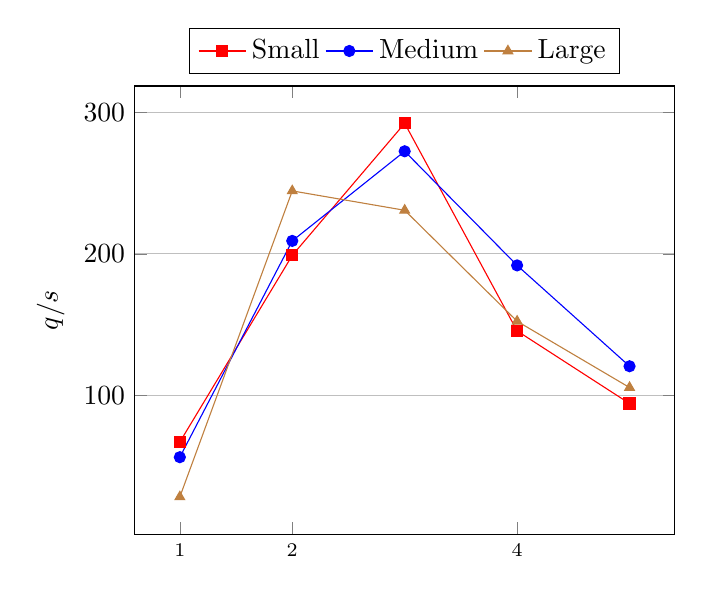
\begin{tikzpicture}
\begin{axis}[
ylabel=$q/s$,
x tick label style={font=\scriptsize},
legend style={at={(0.5,1.13)}, anchor=north, legend columns=-1},
xtick={1,2,4,8,16},
%ybar,
ymajorgrids=true,
%bar width=5pt,
]

\addplot[red,mark=square*]
coordinates {(1, 66.884) (2, 198.906) (3, 292.334) (4, 145.492) (5, 94.124)};
\addplot[blue,mark=*]
%coordinates {(1, 56.163) (2, 209.161) (3, 272.554) (4, 31.234) (5, 120.493)};
coordinates {(1, 56.163) (2, 209.161) (3, 272.554) (4, 191.828) (5, 120.493)};
\addplot[brown,mark=triangle*]
coordinates {(1, 28.062) (2, 244.529) (3, 230.814) (4, 152.311) (5, 105.441)};

\legend{Small, Medium, Large}

\end{axis}
\end{tikzpicture}%

  	}
  	\label{fig:low-query-rate}
  }\quad%
  \subfloat[Query rate with MH selectivity]{%
    \resizebox{0.45\linewidth}{!}{%
      
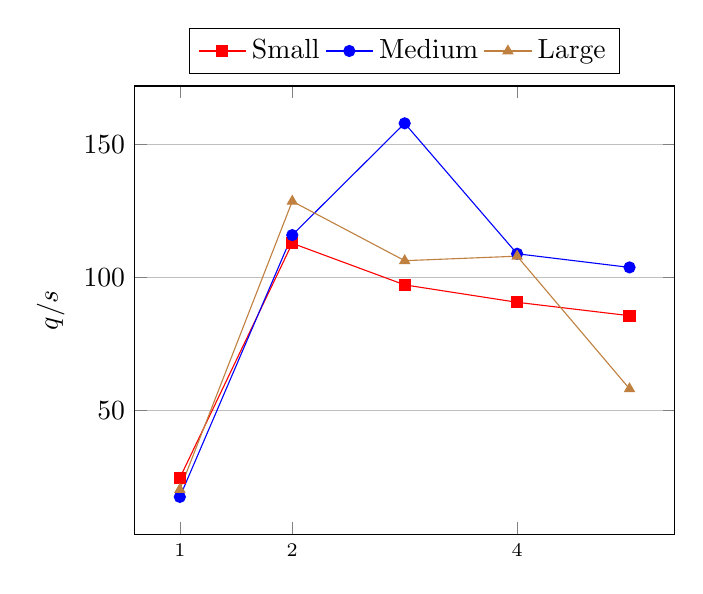
\begin{tikzpicture}
\begin{axis}[
ylabel=$q/s$,
x tick label style={font=\scriptsize},
legend style={at={(0.5,1.13)}, anchor=north, legend columns=-1},
xtick={1,2,4,8},
%ybar,
ymajorgrids=true,
%bar width=5pt,
]

\addplot[red,mark=square*]
coordinates {(1, 24.614) (2, 112.895) (3, 97.257) (4, 90.697) (5, 85.659)};
\addplot[blue,mark=*]
coordinates {(1, 17.492) (2, 115.986) (3, 158.028) (4, 108.956) (5, 103.826)};
\addplot[brown,mark=triangle*]
coordinates {(1, 20.265) (2, 128.696) (3, 106.352) (4, 108.047) (5, 58.153)};

\legend{Small, Medium, Large}

\end{axis}
\end{tikzpicture}%

    }
    \label{fig:medium-query-rate}
  }%
	\caption{The evolution of the average query rate with respect to the size of the star queries over different dataset size.}
	\label{fig:query-rate}
\end{figure}

\section{Discussion}

While AFOR provides better compression ratio than PFOR, AFOR-2 is slower than
PFOR on position file, suggesting that PFOR exception management is slightly
more efficient than the variable frame length approach of AFOR-2 on very
sparse lists. The number of table lookups in AFOR-2 costs more than the
decoding and patching of the exceptions in PFOR.

In general, FOR even if it has more data to read and decompress still provides
the best query execution time. The reason is that our experiments are
performed using warm cache. We therefore ignore the cost of disk IO
accesses and so we can expect a drop of performance for algorithms with a low
compression ratio such as FOR and PFOR compared to AFOR when executing with a
cold cache.

% Compression and decompression performance do not only depend on the
% compression ratio, but also on the execution flow of the algorithm and the
% number of cycles needed to compress or decompress an integer. Therefore,
% CPU-optimised algorithms providing good compression ratio increase the update
% and query throughputs of web search engines. In that context, AFOR seems to be
% a good candidate since it is well balanced in all aspects: it provides very
% good indexing and querying performance and one of the best compression ratio.
% 
% The Simple encoding family is somehow similar to AFOR. At each iteration, S-64
% encodes or decodes a variable number of integers using CPU optimised routines.
% AFOR is however not tied to the machine words, is simpler to implement and
% provides better compression ratio, compression speed and decompression speed.
